\chapter{Experimentos}
\thispagestyle{empty}

\section{Entorno de desarrollo}

El proyecto se llevó a cabo utilizando exclusivamente el lenguaje de programación \textit{Python} en su versión 3.11.8, debido a su versatilidad y eficacia en diversas áreas, desde el renderizado de modelos 3D en \textit{Blender} hasta el desarrollo de modelos de aprendizaje profundo. Se emplearon diversas bibliotecas para diferentes tareas: \textit{Trimesh} y \textit{PyVista} junto con \textit{VTK} para la manipulación de modelos 3D; \textit{Mediapipe} para la extracción de puntos de referencia faciales; \textit{NumPy} y \textit{pandas} para el procesamiento de datos; \textit{PIL} para el trabajo con imágenes; \textit{matplotlib} y \textit{Seaborn} para la generación de gráficos; \textit{Optuna} para la optimización de hiperparámetros; \textit{MLflow} para la gestión de experimentos; y, finalmente, \textit{PyTorch} en su versión 2.0.1 junto con las librerías CUDA para el entrenamiento de modelos de aprendizaje profundo.

Con el objetivo de realizar un control de versiones durante el desarrollo del proyecto, se utilizó Git junto con GitHub. El código generado se puede encontrar en el siguiente enlace \url{https://github.com/ivansalinasugr/TFG}. Para más información, consultar el Readme del repositorio.

\section{Entorno de ejecución}

El proceso de ejecución se lleva a cabo en un entorno de alto rendimiento ubicado en la Universidad de Granada, al que se accede de forma remota a través de SSH. Se emplea un script de Shell para configurar los parámetros esenciales de los archivos. Por un lado, se utiliza SLURM para reservar recursos en la partición \enquote*{dios} del clúster, asignando una GPU del nodo \enquote*{dionisio}. Este nodo cuenta con dos Quadro RTX 8000, una memoria RAM de 512 GB DDR4 y dos procesadores Intel Xeon Silver 4216. Por otro lado, Conda se encarga de gestionar el entorno de software, garantizando la disponibilidad de las bibliotecas necesarias durante el proceso.

\section{Resultados}

En este trabajo se realizarán varios experimentos para entrenar y validar los dos modelos de aprendizaje presentados en FacialSCDnet+. Antes de los entrenamientos, se llevará a cabo un ajuste de parámetros para optimizar el rendimiento de los modelos. Finalmente, se compararán los resultados obtenidos con los obtenidos por FacialSCDnet. Estas comparaciones se efectuarán mediante el rendimiento en dos conjuntos de imágenes: el conjunto de test sintético de FacialSCDnet+, y el conjunto real de FacialSCDnet. Esto nos permitirá evaluar la robustez y la capacidad de generalización de los modelos propuestos.

El objetivo de estos experimentos es validar la hipótesis de que los modelos presentados en este trabajo pueden igualar o superar el rendimiento del modelo de referencia y por tanto, estimar mejor la SCD en fotografías faciales. A continuación, se presentan los detalles específicos y los resultados de estos experimentos.

\subsection{Ajuste de hiperparámetros}

Inicialmente, se llevó a cabo una fase de ajuste de hiperparámetros con el fin de determinar una configuración óptima para las arquitecturas propuestas. Los rangos de valores y los parámetros finales se detallan en la Tabla \ref{hipertuneo}. Además de los hiperparámetros mencionados, se estableció un entrenamiento a lo largo de 300 épocas, con una tasa de aprendizaje mínima de $10^{-12}$ y una reducción de la tasa de aprendizaje del 20\% cada 3 épocas consecutivas sin mejoras (paciencia), hasta un mínimo de $10^{-12}$.

\begin{table}[h]
	\centering
	\resizebox{\textwidth}{!}{%
	\begin{tabular}{llll}
	\hline
	Parámetros & Opciones & Mejor VGG-16 & Mejor ResNet-50 \\ \hline
	Optimizador & [adam, sgd] & adam & adam \\
	Tasa de aprendizaje & [$10^{-6}$, $10^{-3}$] & $4.63 \cdot 10^{-5}$ & 0.00042 \\
	Tamaño del lote & [16, 32, 64, 128] & 32 & 32 \\
	Paciencia & [2, 3, 4] & 3 & 3 \\
	\textit{Early Stopping} & [4, 6, 8] & 6 & 6 \\
	\textit{Dropout} (\%) & [0, 10, 20, 30] & 0 & 0 \\ \hline
	\end{tabular}%
	}
	\caption[Selección de parámetros de entrenamiento FacialSCDnet+.]{Parámetros de entrenamiento seleccionados para las redes VGG-16 y ResNet-50, junto a los rangos de valores utilizados durante el proceso de optimización de hiperparámetros.}
	\label{hipertuneo}
\end{table}

Los detalles de implementación de este tuneo de hiperparámetros se pueden observar en la Sección \ref{sec-hipertuneo}.

\subsection{Comparativa Arquitecturas}

A continuación, para valorar el comportamiento de las diferentes arquitecturas propuestas, compararemos los resultados obtenidos para FacialSCDnet+ usando el conjunto de validación. La Figura \ref{fig30} muestra la gráfica de la función de pérdida durante el entrenamiento de ambas arquitecturas, mientras que la Tabla \ref{val-metrics} muestra los valores finales de las métricas en el conjunto de entrenamiento de validación tras finalizar el entrenamiento.

\begin{figure}[h]
	\centering
	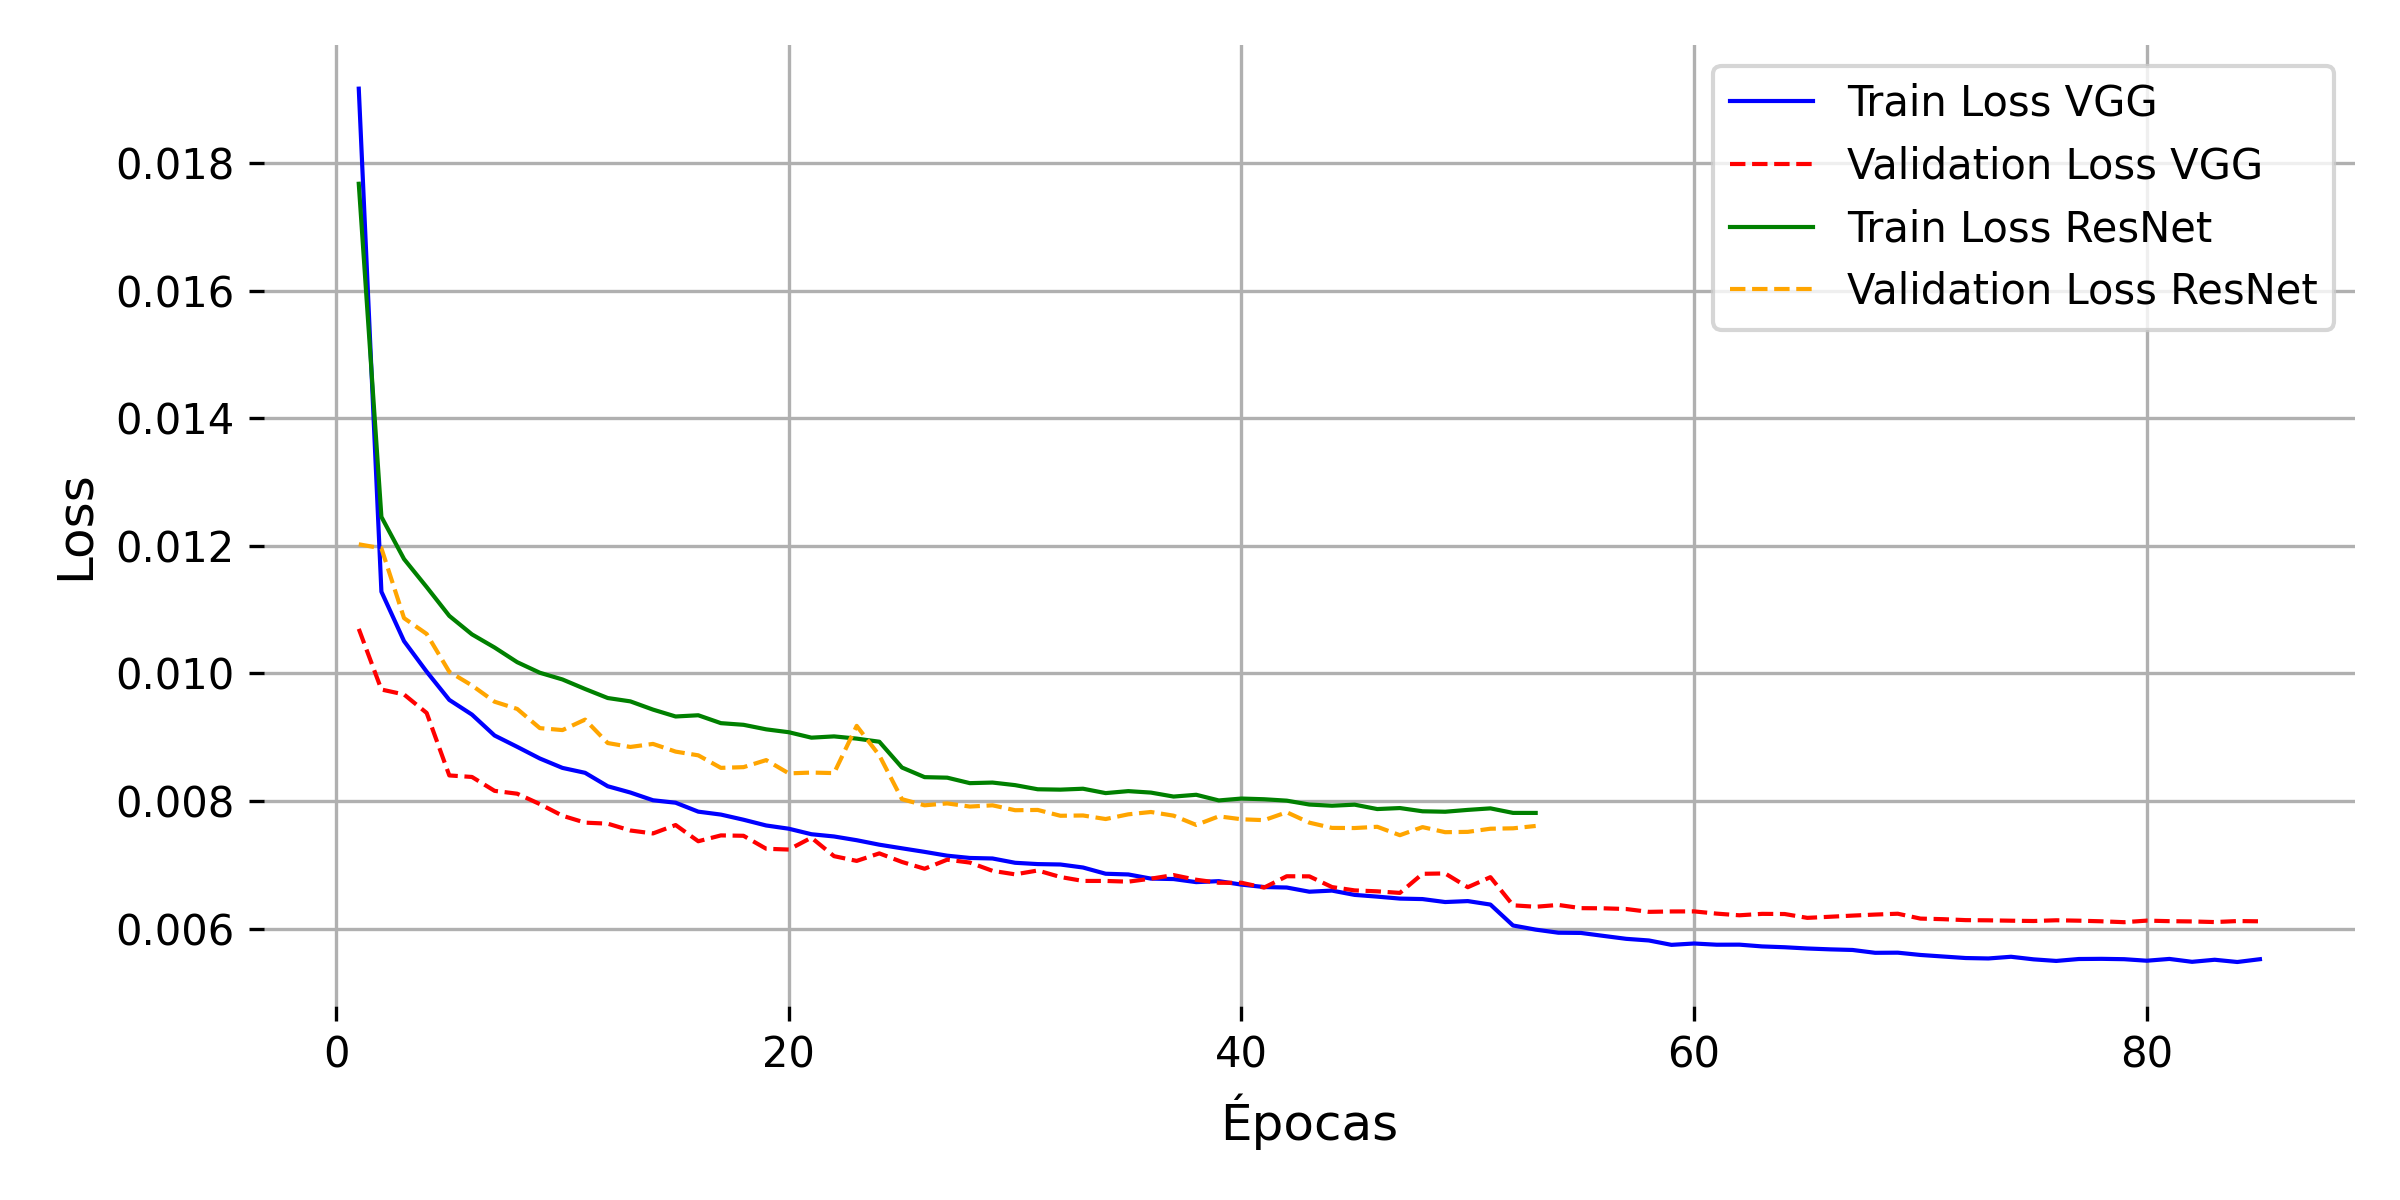
\includegraphics[scale=0.6]{imagenes/cap5/train_val_loss.png}
	\caption[Gráfica de pérdida en entrenamiento y validación.]{Gráfica de la función de pérdida durante el entrenamiento de las redes VGG-16 y ResNet-50. Para la red VGG se representa en azul la pérdida en el conjunto de entrenamiento mientras que en rojo se representa la pérdida en el conjunto de validación. Para la red ResNet se representa en verde la pérdida en el conjunto de entrenamiento mientras que en naranja se representa la pérdida en el conjunto de validación.}
	\label{fig30}
\end{figure}

Ambas arquitecturas comienzan con una pérdida alta que disminuye rápidamente durante las primeras épocas, lo cual es esperado ya que los modelos empiezan a ajustarse a los datos de entrenamiento. A medida que avanza el entrenamiento, ambos modelos van aprendiendo de los datos y por tanto, las pérdidas de entrenamiento y de validación siguen disminuyendo. 

VGG-16 muestra una convergencia más suave y una pérdida más baja tanto en entrenamiento como en validación en comparación con ResNet-50. Aunque ResNet-50 comienza bien, alcanza una meseta en la reducción de la pérdida de entrenamiento más rápidamente que VGG-16. Por tanto, la arquitectura VGG-16 tiene un mejor rendimiento en términos de pérdida tanto en entrenamiento como en validación en comparación con ResNet-50. 

Además, ambas arquitecturas finalizan el entrenamiento debido al \textit{early stopping}, tras seis épocas sin mejorar. La aplicación de esta técnica parece haber sido efectiva, ya que no se observa una gran divergencia entre las pérdidas de entrenamiento y validación hacia el final de la gráfica. Esto indica que los modelos no están sobreajustando significativamente y mantienen un buen equilibrio entre el ajuste a los datos de entrenamiento y la capacidad de generalización.

\begin{table}[h]
	\centering
	\resizebox{\textwidth}{!}{%
	\begin{tabular}{llll}
	\hline
	Métricas de evaluación &  & Validación VGG-16 & Validación ResNet-50 \\ \hline
	Distorsión (\%) &
	  \begin{tabular}[c]{@{}l@{}}Media (std)\\ Mediana\\ Perc 90, 95, 99\end{tabular} &
	  \begin{tabular}[c]{@{}l@{}}\textbf{0.61} (\textbf{0.614})\\ \textbf{0.434}\\ {[}\textbf{1.356}, \textbf{1.747}, \textbf{2.742}{]}\end{tabular} &
	  \begin{tabular}[c]{@{}l@{}}0.746 (0.722)\\ 0.532\\ {[}1.692, 2.176, 3.266{]}\end{tabular} \\ \hline
	MAE (cm) &
	  \begin{tabular}[c]{@{}l@{}}Media (std)\\ Mediana\\ Perc 90, 95, 99\end{tabular} &
	  \begin{tabular}[c]{@{}l@{}}\textbf{31.425} (44.048)\\ \textbf{12.194}\\ {[}\textbf{89.95}, \textbf{125.106}, 204.385{]}\end{tabular} &
	  \begin{tabular}[c]{@{}l@{}}34.072 (\textbf{43.447})\\ 15.597\\ {[}93.849, 126.878, \textbf{194.479}{]}\end{tabular} \\ \hline
	MRE (\%) &
	  \begin{tabular}[c]{@{}l@{}}Media (std)\\ Mediana\\ Perc 90, 95, 99\end{tabular} &
	  \begin{tabular}[c]{@{}l@{}}\textbf{0.111} (0.138)\\ \textbf{0.075}\\ {[}\textbf{0.233}, \textbf{0.328}, \textbf{0.647}{]}\end{tabular} &
	  \begin{tabular}[c]{@{}l@{}}0.128 (\textbf{0.137})\\ 0.093\\ {[}0.266, 0.356, 0.659{]}\end{tabular} \\ \hline
	R$^2$ &
	  &
	  \textbf{0.897} &
	  0.894 \\ \hline
	\end{tabular}%
	}
	\caption[Métricas en validación VGG-16 y ResNet-50.]{Métricas en el conjunto de validación tras el proceso de entrenamiento de las redes VGG-16 y ResNet-50.}
	\label{val-metrics}
\end{table}

A pesar de que los valores del MAE son relativamente altos, ambos modelos muestran un error medio de distorsión menor al 1\% y un error relativo medio muy bajo, lo cual es un valor aceptable para que la predicción sea fiable. En este contexto, VGG-16 presenta una distorsión ligeramente más baja que ResNet-50, lo que indica una mejor predicción de las distancias.

En general, aunque ambos modelos tienen buenos resultados, sobre todo en términos de distorsión, VGG-16 destaca con mejor rendimiento que ResNet-50 en todas las métricas.

\subsection{Comparativa con el estado del arte: FacialSCDnet}

En esta sección se lleva a cabo una comparativa entre los tres modelos utilizados para la estimación de la SCD: VGG-16 y ResNet-50 de FacialSCDnet+ y VGG-16 de FacialSCDnet. Para ello, se evalúan los modelos en dos conjuntos de datos: el conjunto de test sintético propuesto en este trabajo, previamente definido en la Sección \ref{protocolo} y un conjunto de test de imágenes reales propuesto en \cite{14}. Así, se pretende proporcionar una comparativa en igualdad de condiciones para ambos métodos. 

Aunque no se deberían utilizar los conjuntos de test para tomar decisiones metodológicas debido al riesgo de \textit{data snooping} (lo que puede llevar a un sobreajuste a los datos de test), en este trabajo seguiremos el protocolo del estudio de referencia \cite{14} y de muchos otros estudios, utilizando los conjuntos de test para evaluar y comparar el rendimiento de los modelos.

Para hacer la comparación más visual, se complementarán las métricas con figuras que muestren las predicciones comparadas con los valores objetivo, así como los errores de predicción representados en diagramas de caja.

\subsubsection{Test imágenes sintéticas}

Este conjunto de datos contiene 28 935 imágenes sintéticas en 35 distancias desde 50 a 600 cm. Los resultados de evaluar los modelos en este conjunto de datos se muestran en la Tabla \ref{test-mio}.

\begin{table}[h]
	\centering
	\resizebox{\textwidth}{!}{%
	\begin{tabular}{lllll}
	\hline
	\begin{tabular}[c]{@{}l@{}}Métricas de \\ evaluación\end{tabular} &
	&
	\begin{tabular}[c]{@{}l@{}}VGG-16 \\ FSCDnet\end{tabular} &
	\begin{tabular}[c]{@{}l@{}}VGG-16 \\ FSCDnet+\end{tabular} &
	\begin{tabular}[c]{@{}l@{}}ResNet-50 \\ FSCDnet+\end{tabular} \\ \hline
	Distorsión (\%) &
	\begin{tabular}[c]{@{}l@{}}Media (std)\\ Mediana\\ Perc 90, 95, 99\end{tabular} &
	\begin{tabular}[c]{@{}l@{}}1.218 (1.395)\\ 0.764\\ {[}2.878, 3.893, 6.826{]}\end{tabular} &
	\begin{tabular}[c]{@{}l@{}}\textbf{0.624} (\textbf{0.596})\\ \textbf{0.453}\\ {[}\textbf{1.381}, \textbf{1.758}, \textbf{2.639}{]}\end{tabular} &
	\begin{tabular}[c]{@{}l@{}}0.781 (0.754)\\ 0.55\\ {[}1.782, 2.265, 3.445{]}\end{tabular} \\ \hline
	MAE (cm) &
	\begin{tabular}[c]{@{}l@{}}Media (std)\\ Mediana\\ Perc 90, 95, 99\end{tabular} &
	\begin{tabular}[c]{@{}l@{}}53.237 (73.434)\\ 21.594\\ {[}147.604, 220.045, 338.481{]}\end{tabular} &
	\begin{tabular}[c]{@{}l@{}}\textbf{32.165} (44.045)\\ \textbf{12.771}\\ {[}\textbf{92.037}, \textbf{127.188}, 200.073{]}\end{tabular} &
	\begin{tabular}[c]{@{}l@{}}35.095 (\textbf{43.954})\\ 16.498\\ {[}96.793, 130.566, \textbf{193.916}{]}\end{tabular} \\ \hline
	MRE (\%) &
	\begin{tabular}[c]{@{}l@{}}Media (std)\\ Mediana\\ Perc 90, 95, 99\end{tabular} &
	\begin{tabular}[c]{@{}l@{}}0.215 (0.299)\\ 0.132\\ {[}0.455, 0.681, 1.567{]}\end{tabular} &
	\begin{tabular}[c]{@{}l@{}}\textbf{0.113} (\textbf{0.135})\\ \textbf{0.078}\\ {[}\textbf{0.24}, \textbf{0.327}, \textbf{0.64}{]}\end{tabular} &
	\begin{tabular}[c]{@{}l@{}}0.133 (0.14)\\ 0.099\\ {[}0.277, 0.362, 0.669{]}\end{tabular} \\ \hline
	R$^2$ &
	&
	0.673 &
	\textbf{0.895} &
	0.89 \\ \hline
	\end{tabular}%
	}
	\caption[Métricas en el conjunto de test sintético.]{Métricas en el conjunto de test sintético de FacialSCDnet+, comparando los modelos VGG-16 y ResNet-50 de FacialSCDnet+ contra el modelo de FacialSCDnet.}
	\label{test-mio}
\end{table}

Esta tabla refleja cómo VGG-16 FacialSCDnet+ presenta mejores resultados en la mayoría de las métricas, seguido por ResNet-50 FacialSCDnet+ y VGG-16 FacialSCDnet. Estos resultados sugieren que el método FacialSCDnet+ proporciona una mejora significativa en el rendimiento de la predicción en comparación con el método FacialSCDnet, y se reafirma la conclusión obtenida en la comparativa anterior, donde la arquitectura de VGG-16 se comporta mejor que ResNet-50 en este contexto específico.

Ambos modelos de FacialSCDnet+ presentan una distorsión inferior al 1\%, lo cual se considera un margen de error aceptable, incluso a pesar de que muestran un MAE elevado. Visualmente, podemos analizar la distribución del error en la Figura \ref{fig33}, donde se compara el error en las predicciones mediante gráficos de caja.

\begin{figure}[h]
	\centering
	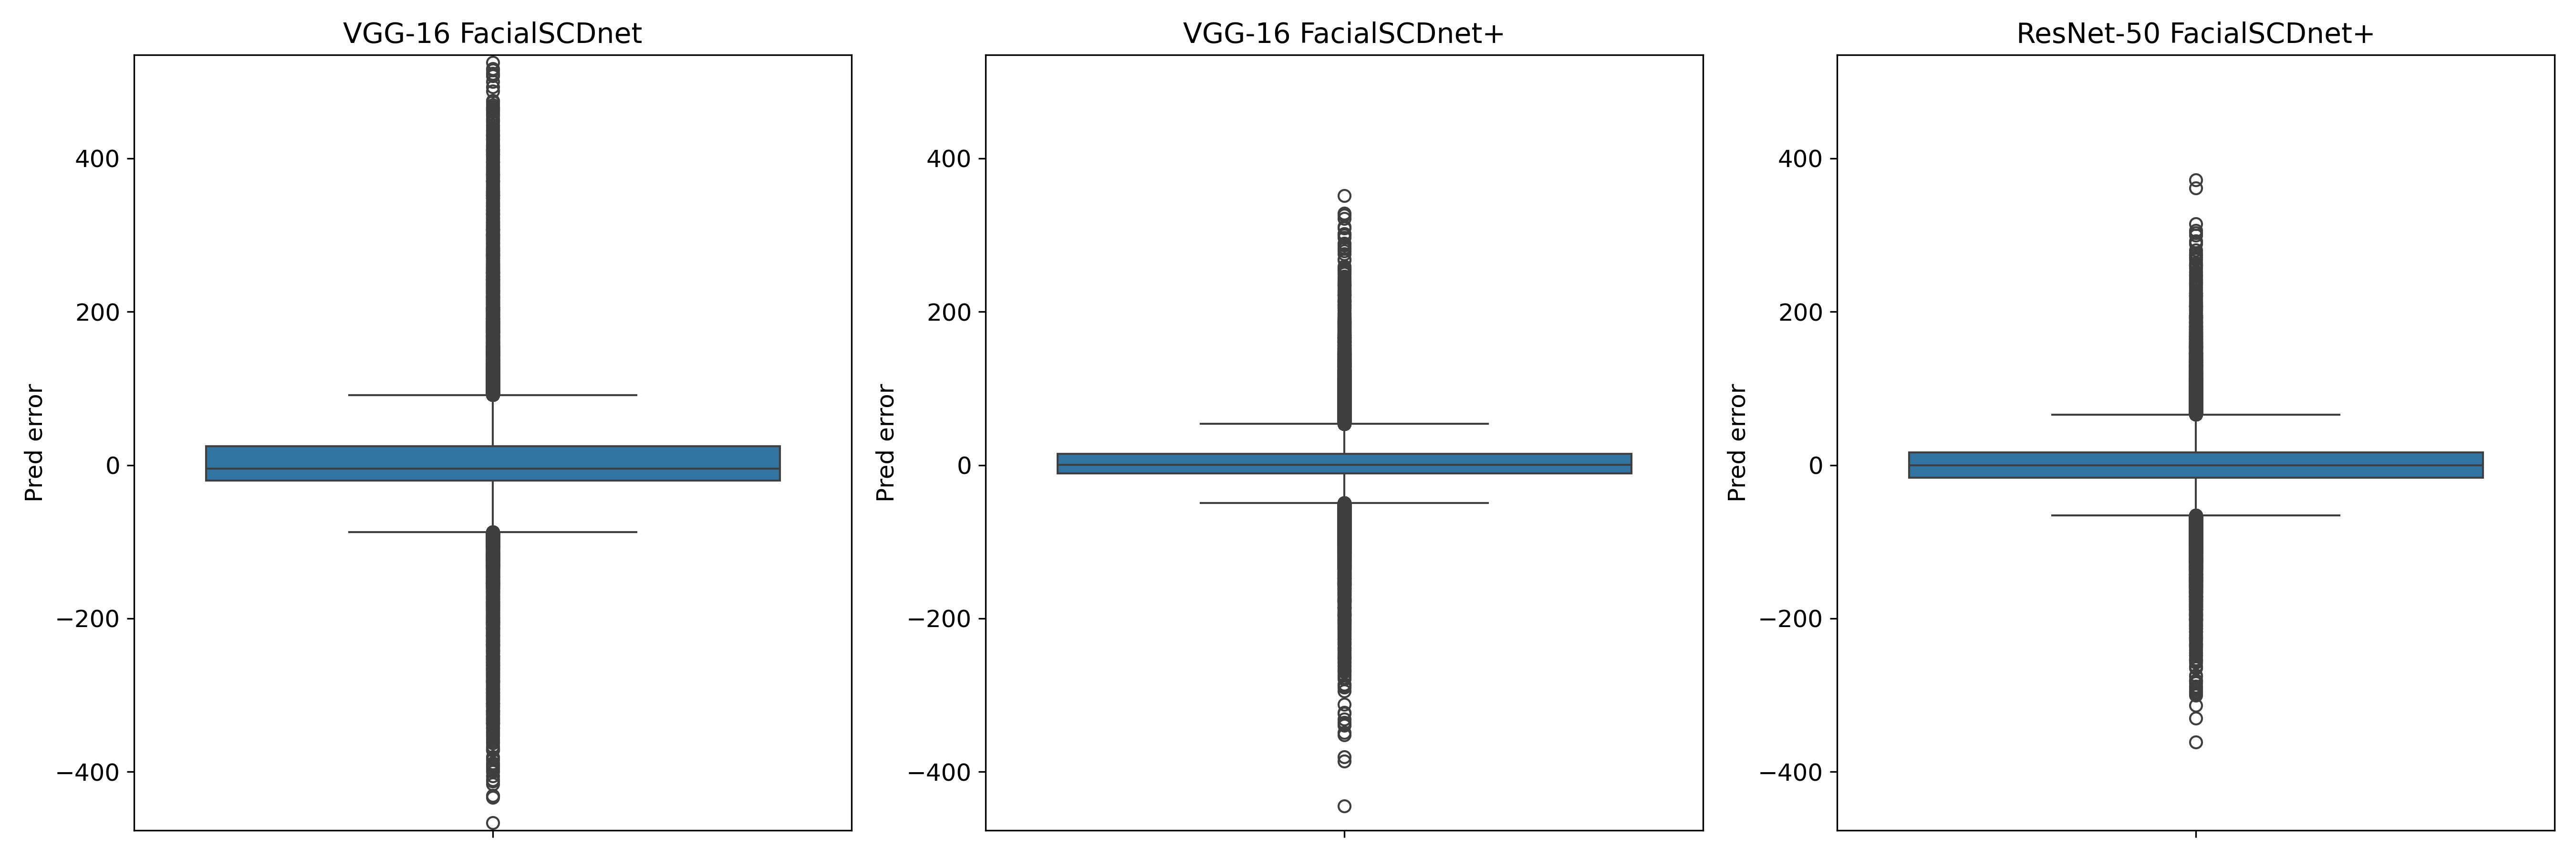
\includegraphics[width=\textwidth]{imagenes/cap5/boxplot_own.png}
	\caption[Comparación predicciones de error test sintético.]{Gráfica que muestra la comparación de las predicciones de error para cada uno de los 3 modelos utilizados.}
	\label{fig33}
\end{figure}

En estas gráficas se puede observar cómo VGG-16 FacialSCDnet muestra la mayor variabilidad y la mayor cantidad de outliers, lo que sugiere que este modelo enfrenta más dificultades para hacer predicciones precisas en muchos casos. Los dos modelos de FacialSCDnet+ mejoran en comparación con FacialSCDnet, reduciendo tanto la variabilidad como la cantidad de outliers, lo que indica un desempeño más consistente. En particular, el modelo VGG-16 FacialSCDnet+ parece tener menor variabilidad, mientras que ResNet-50 presenta la menor cantidad de outliers.

En la Figura \ref{fig36} se pueden observar predicciones de la distancia para algunas de las imágenes del conjunto sintético.

\begin{figure}[h]
	\centering
	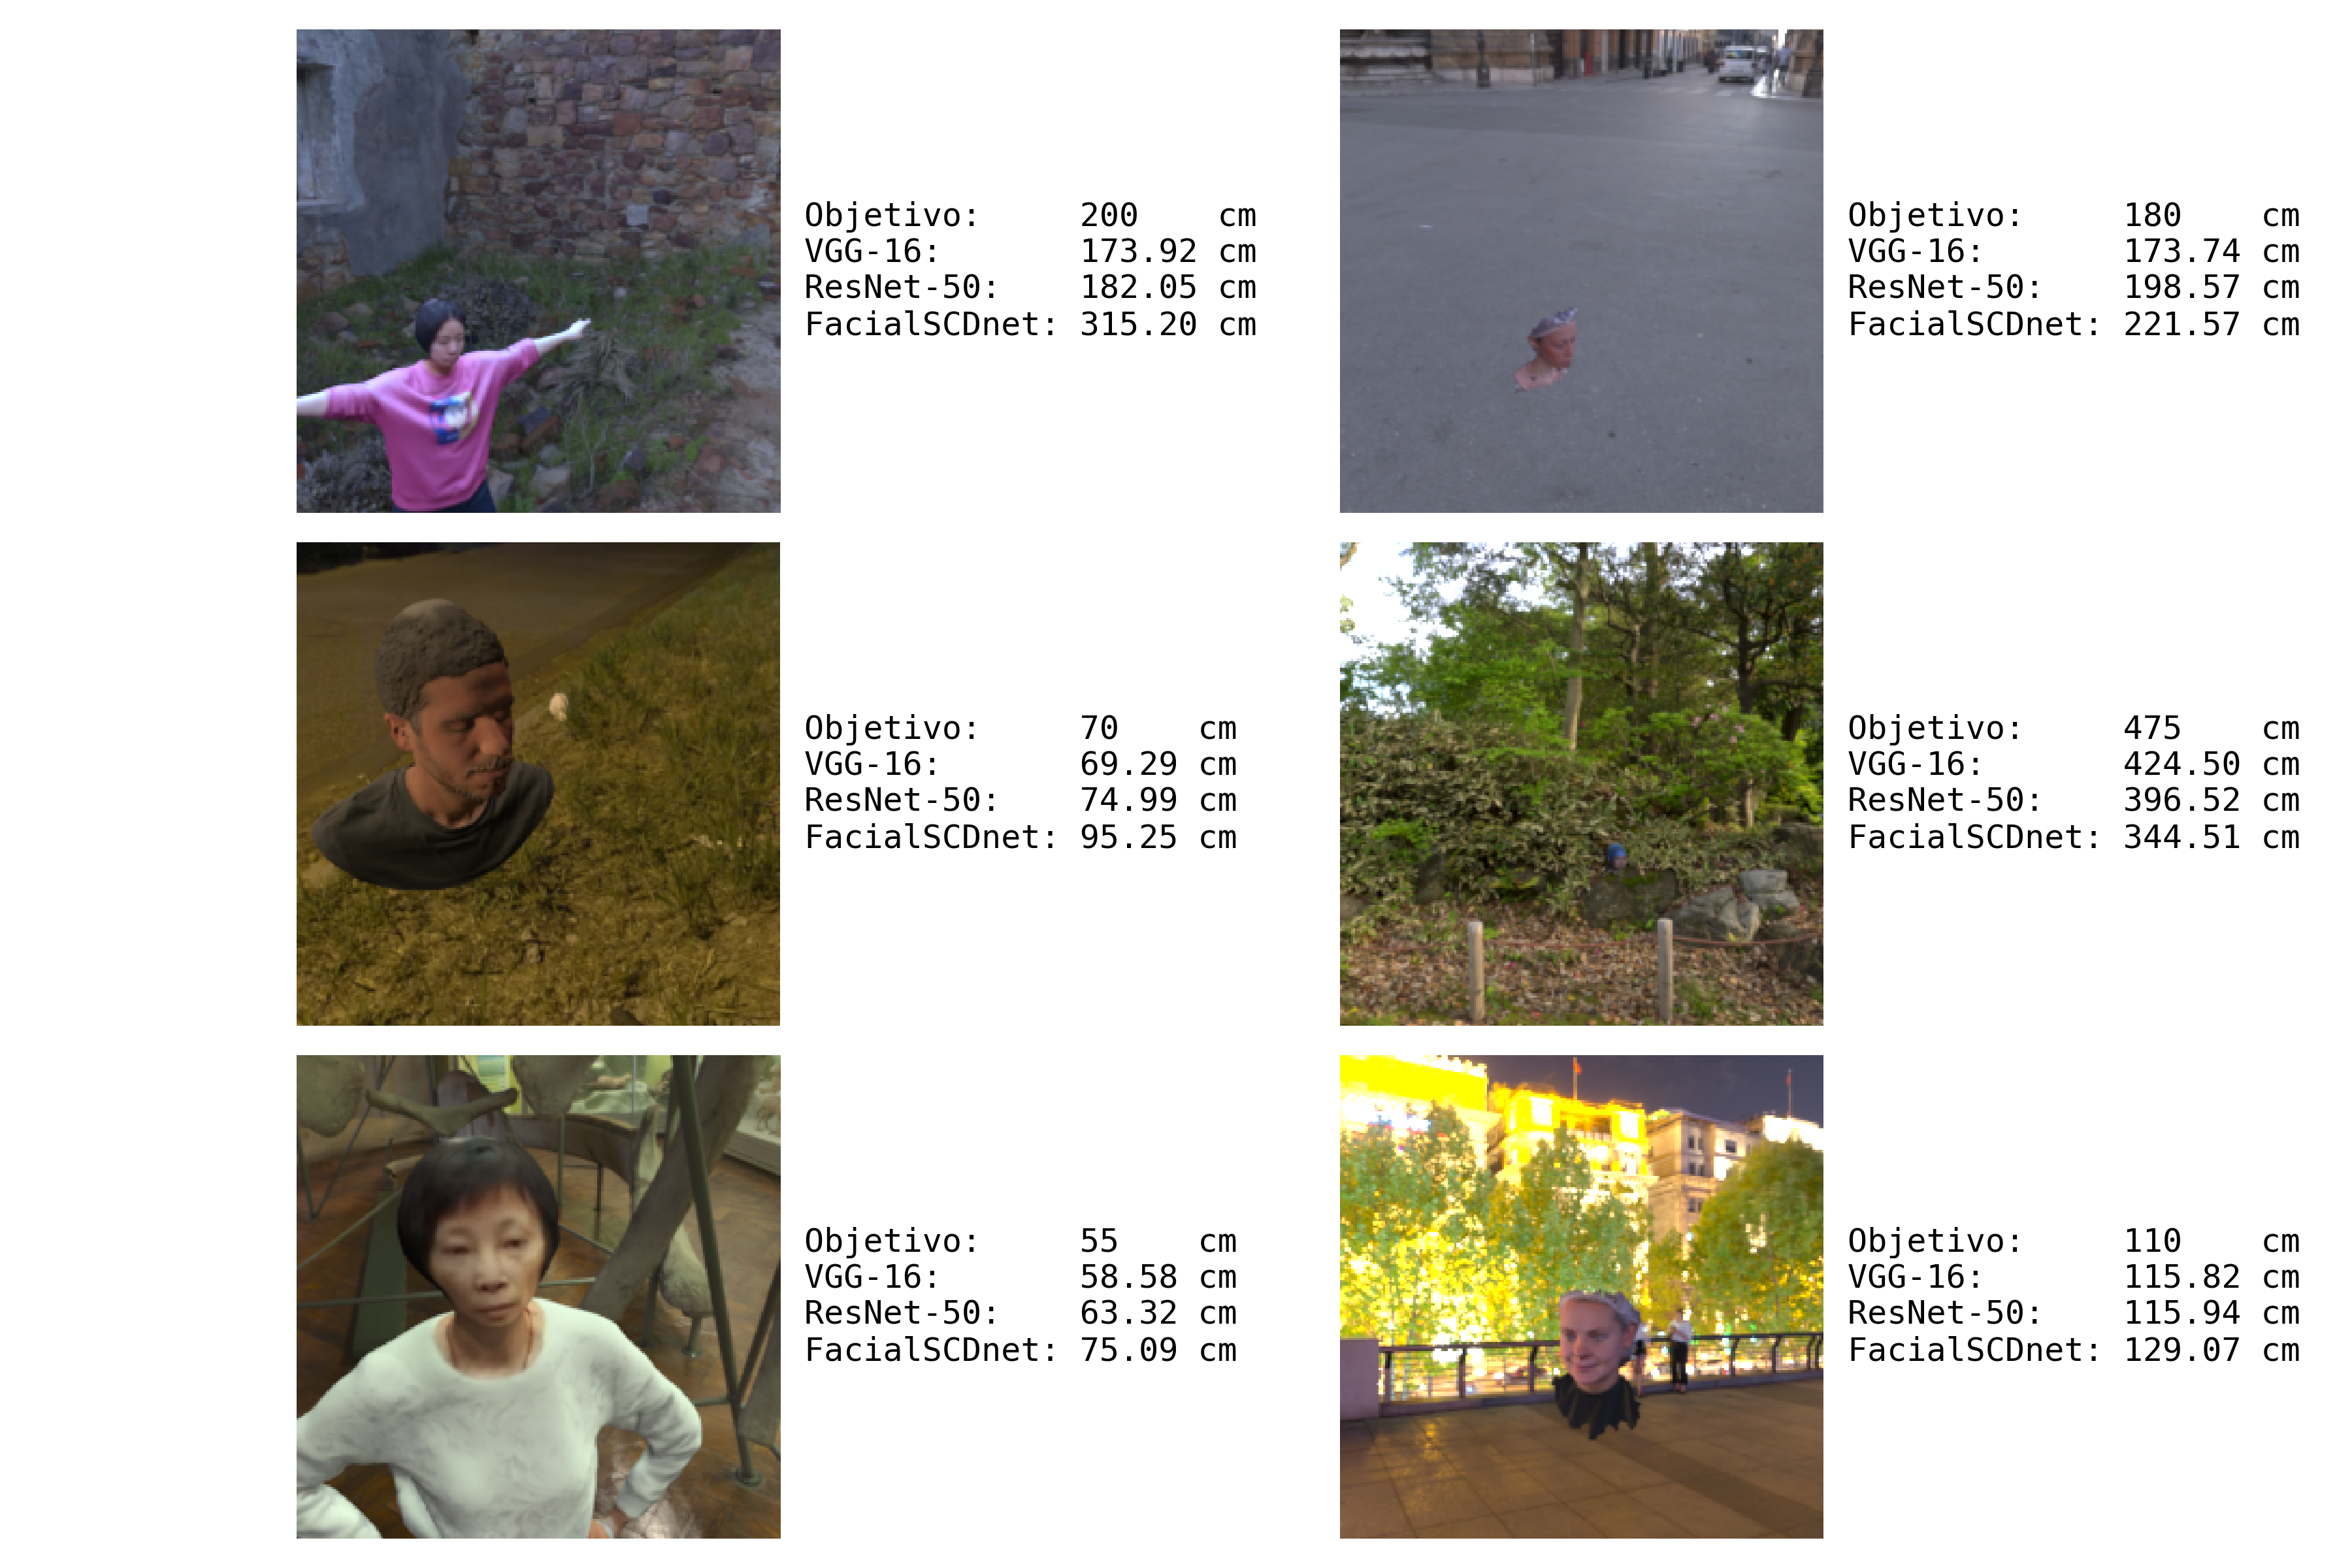
\includegraphics[width=\textwidth]{imagenes/cap5/predicts_own.png}
	\caption[Ejemplos de predicciones en imágenes sintéticas.]{Ejemplos de predicciones en imágenes sintéticas para los distintos modelos VGG-16 y ResNet-50 de FacialSCDnet+ y VGG-16 de FacialSCDnet.}
	\label{fig36}
\end{figure}

Es importante destacar que los modelos de FacialSCDnet+ parten con cierta ventaja en esta compartiva, ya que han sido entrenados en un conjunto similar al empleado en este test. Por esta razón, a continuación se evaluarán los modelos en un conjunto de test compuesto únicamente de imágenes reales.


\subsubsection{Test imágenes reales}

Este conjunto de datos contiene 1134 imágenes reales en 29 distancias desde 50 a 500 cm. Los resultados de evaluar los modelos en este conjunto de datos se muestran en la Tabla \ref{test-real}.

\begin{table}[h]
	\centering
	\resizebox{\textwidth}{!}{%
	\begin{tabular}{lllll}
	\hline
	\begin{tabular}[c]{@{}l@{}}Métricas de \\ evaluación\end{tabular} &
	&
	\begin{tabular}[c]{@{}l@{}}VGG-16 \\ FSCDnet\end{tabular} &
	\begin{tabular}[c]{@{}l@{}}VGG-16 \\ FSCDnet+\end{tabular} &
	\begin{tabular}[c]{@{}l@{}}ResNet-50 \\ FSCDnet+\end{tabular} \\ \hline
	Distorsión (\%) &
	\begin{tabular}[c]{@{}l@{}}Media (std)\\ Mediana\\ Perc 90, 95, 99\end{tabular} &
	\begin{tabular}[c]{@{}l@{}}1.233 (1.615)\\ 0.77\\ {[}3.005, 3.869, 8.389{]}\end{tabular} &
	\begin{tabular}[c]{@{}l@{}}\textbf{0.702} (\textbf{0.727})\\ \textbf{0.477}\\ {[}\textbf{1.637}, \textbf{2.195}, \textbf{3.459}{]}\end{tabular} &
	\begin{tabular}[c]{@{}l@{}}1.257 (0.993)\\ 1.085\\ {[}2.59, 3.136, 4.108{]}\end{tabular} \\ \hline
	MAE (cm) &
	\begin{tabular}[c]{@{}l@{}}Media (std)\\ Mediana\\ Perc 90, 95, 99\end{tabular} &
	\begin{tabular}[c]{@{}l@{}}31.594 (55.366)\\ 9.994\\ {[}98.136, 154.061, 288.525{]}\end{tabular} &
	\begin{tabular}[c]{@{}l@{}}\textbf{26.05} (\textbf{48.391})\\ \textbf{8.69}\\ {[}\textbf{71.072}, \textbf{117.413}, 261.572{]}\end{tabular} &
	\begin{tabular}[c]{@{}l@{}}39.852 (58.581)\\ 16.233\\ {[}130.143, 179.453, \textbf{257.784}{]}\end{tabular} \\ \hline
	MRE (\%) &
	\begin{tabular}[c]{@{}l@{}}Media (std)\\ Mediana\\ Perc 90, 95, 99\end{tabular} &
	\begin{tabular}[c]{@{}l@{}}0.187 (0.33)\\ 0.103\\ {[}0.409, 0.58, 1.61{]}\end{tabular} &
	\begin{tabular}[c]{@{}l@{}}\textbf{0.098} (\textbf{0.101})\\ \textbf{0.067}\\ {[}\textbf{0.212}, \textbf{0.3}, \textbf{0.523}{]}\end{tabular} &
	\begin{tabular}[c]{@{}l@{}}0.161 (0.126)\\ 0.137\\ {[}0.342, 0.409, \textbf{0.523}{]}\end{tabular} \\ \hline
	R$^2$ &
	&
	0.786 &
	\textbf{0.829} &
	0.624 \\ \hline
	\end{tabular}%
	}
	\caption[Métricas en el conjunto de test real.]{Métricas en el conjunto de test real de FacialSCDnet, comparando los modelos VGG-16 y ResNet-50 de FacialSCDnet+ contra el modelo de FacialSCDnet.}
	\label{test-real}
\end{table}

Esta tabla refleja cómo VGG-16 FacialSCDnet+ presenta mejores resultados en todas las métricas, seguido por ResNet-50 FacialSCDnet+ y VGG-16 FacialSCDnet. Esto sugiere que el método FacialSCDnet+ proporciona una mejora significativa en el rendimiento de la predicción en comparación con el método FacialSCDnet estándar, y que el modelo VGG-16 es más efectivo que el ResNet-50 en este contexto específico.

El modelo VGG-16 de FacialSCDnet+ es el único que presenta una distorsión inferior al 1\%. Aunque todavía tiene un MAE ligeramente alto, este nivel de error en la distorsión se considera aceptable.

En este contexto, es notable destacar un error cometido en el método FacialSCDnet. A la hora de evaluar el modelo con las imágenes reales, se les aplicaba una máscara para añadirles un fondo sintético. Esto provocaba que el rendimiento del modelo aumentara artificialmente, ya que la red neuronal internamente estaba aprendiendo a localizar a los individuos en fotografías lejanas gracias al preprocesamiento. Así, se estaba cometiendo un sesgo significativo debido a la aplicación de  máscaras. Los resultados pueden comprobarse en la publicación original \cite{14}, donde se muestran resultados que reducen una sexta parte del error real sin preprocesamiento.

La Figura \ref{fig35} muestra una comparación de las predicciones de error para los tres modelos utilizando gráficos de caja.

\begin{figure}[h]
	\centering
	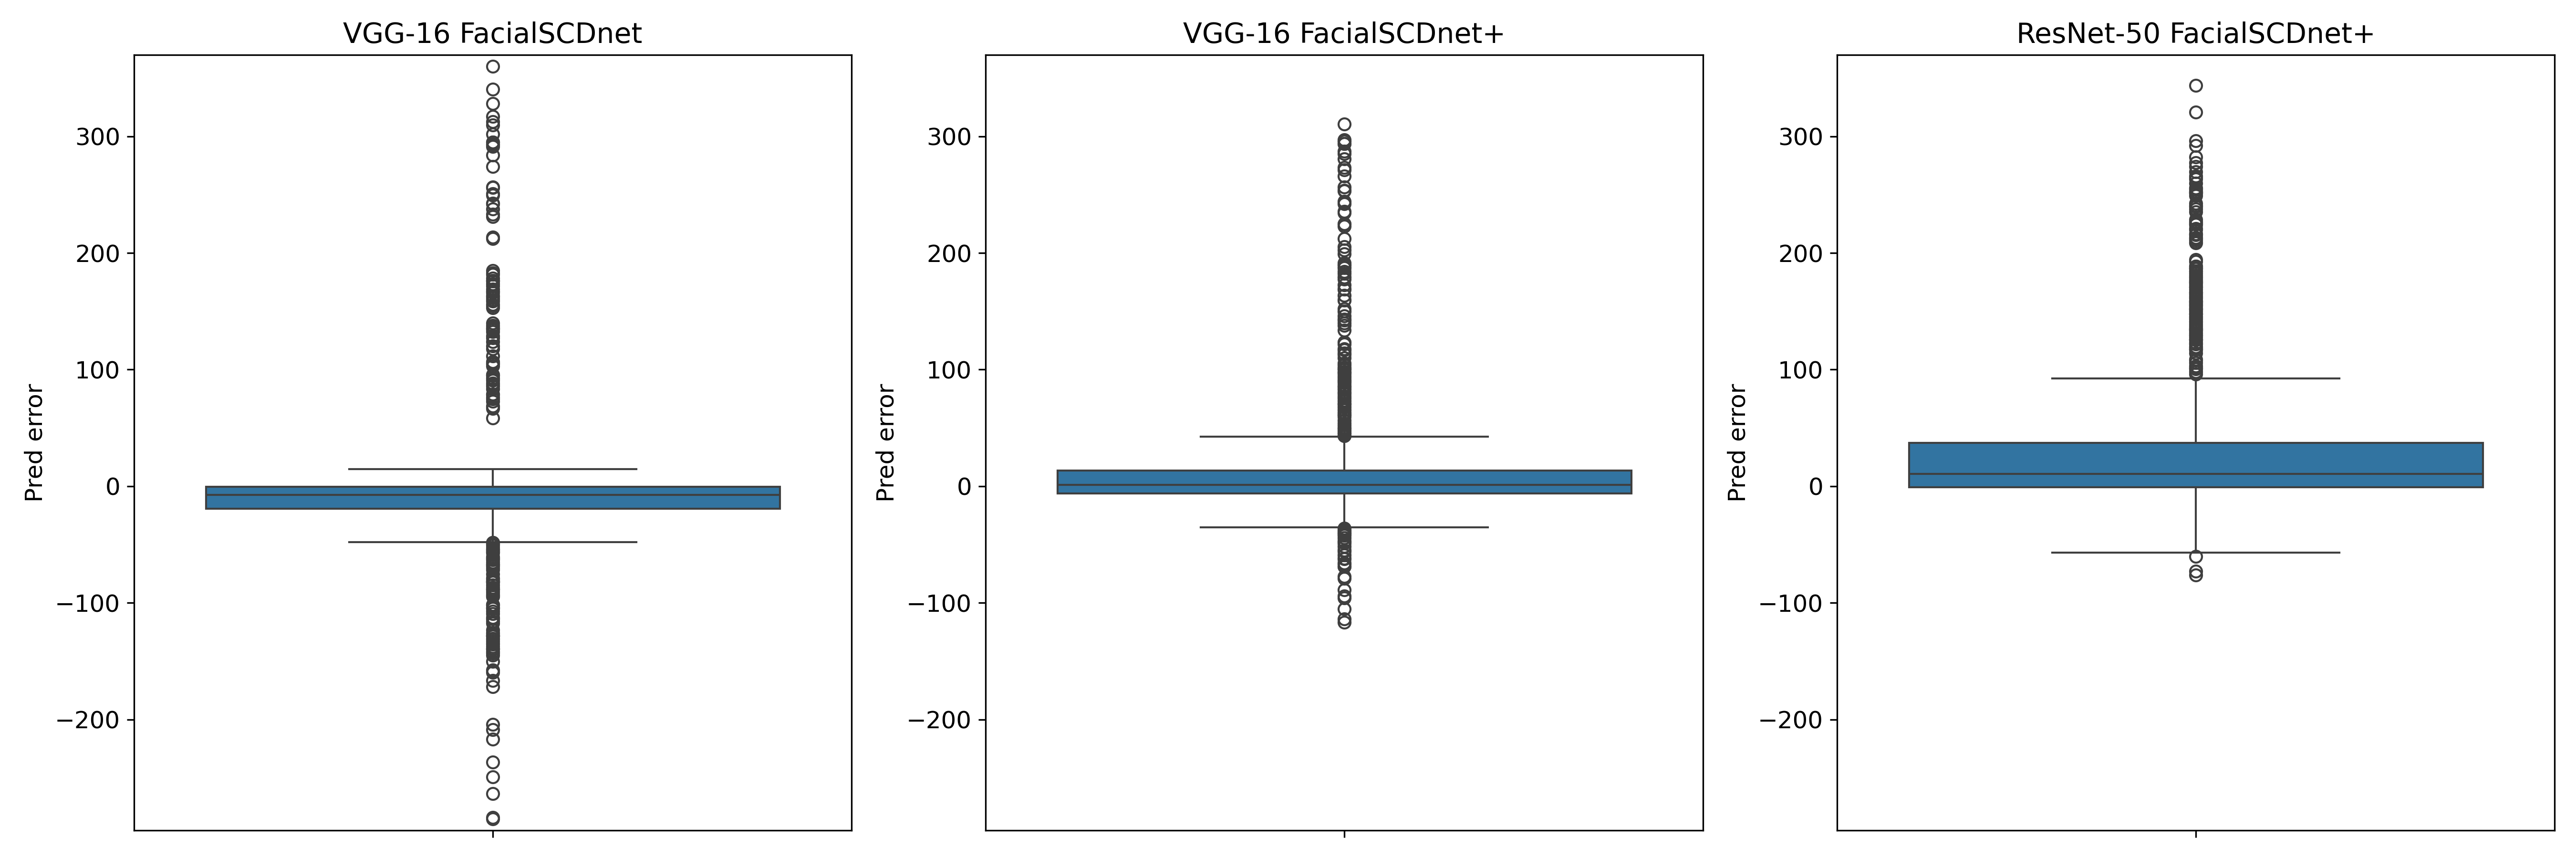
\includegraphics[width=\textwidth]{imagenes/cap5/boxplot_real.png}
	\caption[Comparación predicciones de error test real.]{Gráfica que muestra la comparación de las predicciones de error para cada uno de los 3 modelos utilizados.}
	\label{fig35}
\end{figure}

Se observa que VGG-16 FacialSCDnet presenta la mayor cantidad de outliers, lo que sugiere que este modelo tiene más dificultades para hacer predicciones precisas en ciertos casos. Además, este modelo tiende tanto a sobreestimar como a infraestimar las predicciones. Por otro lado, ambos modelos de FacialSCDnet+ muestran una menor cantidad de outliers, aunque tienen una mayor variabilidad, especialmente el ResNet-50 FacialSCDnet+. El modelo VGG-16 FacialSCDnet+, a pesar de tener una variabilidad ligeramente mayor que el VGG-16 FacialSCDnet, presenta menos outliers, lo cual sugiere que es el modelo más consistente de los presentados.

En la Figura \ref{fig37} se pueden observar predicciones de la distancia para algunas de las imágenes del conjunto real.

\begin{figure}[h]
	\centering
	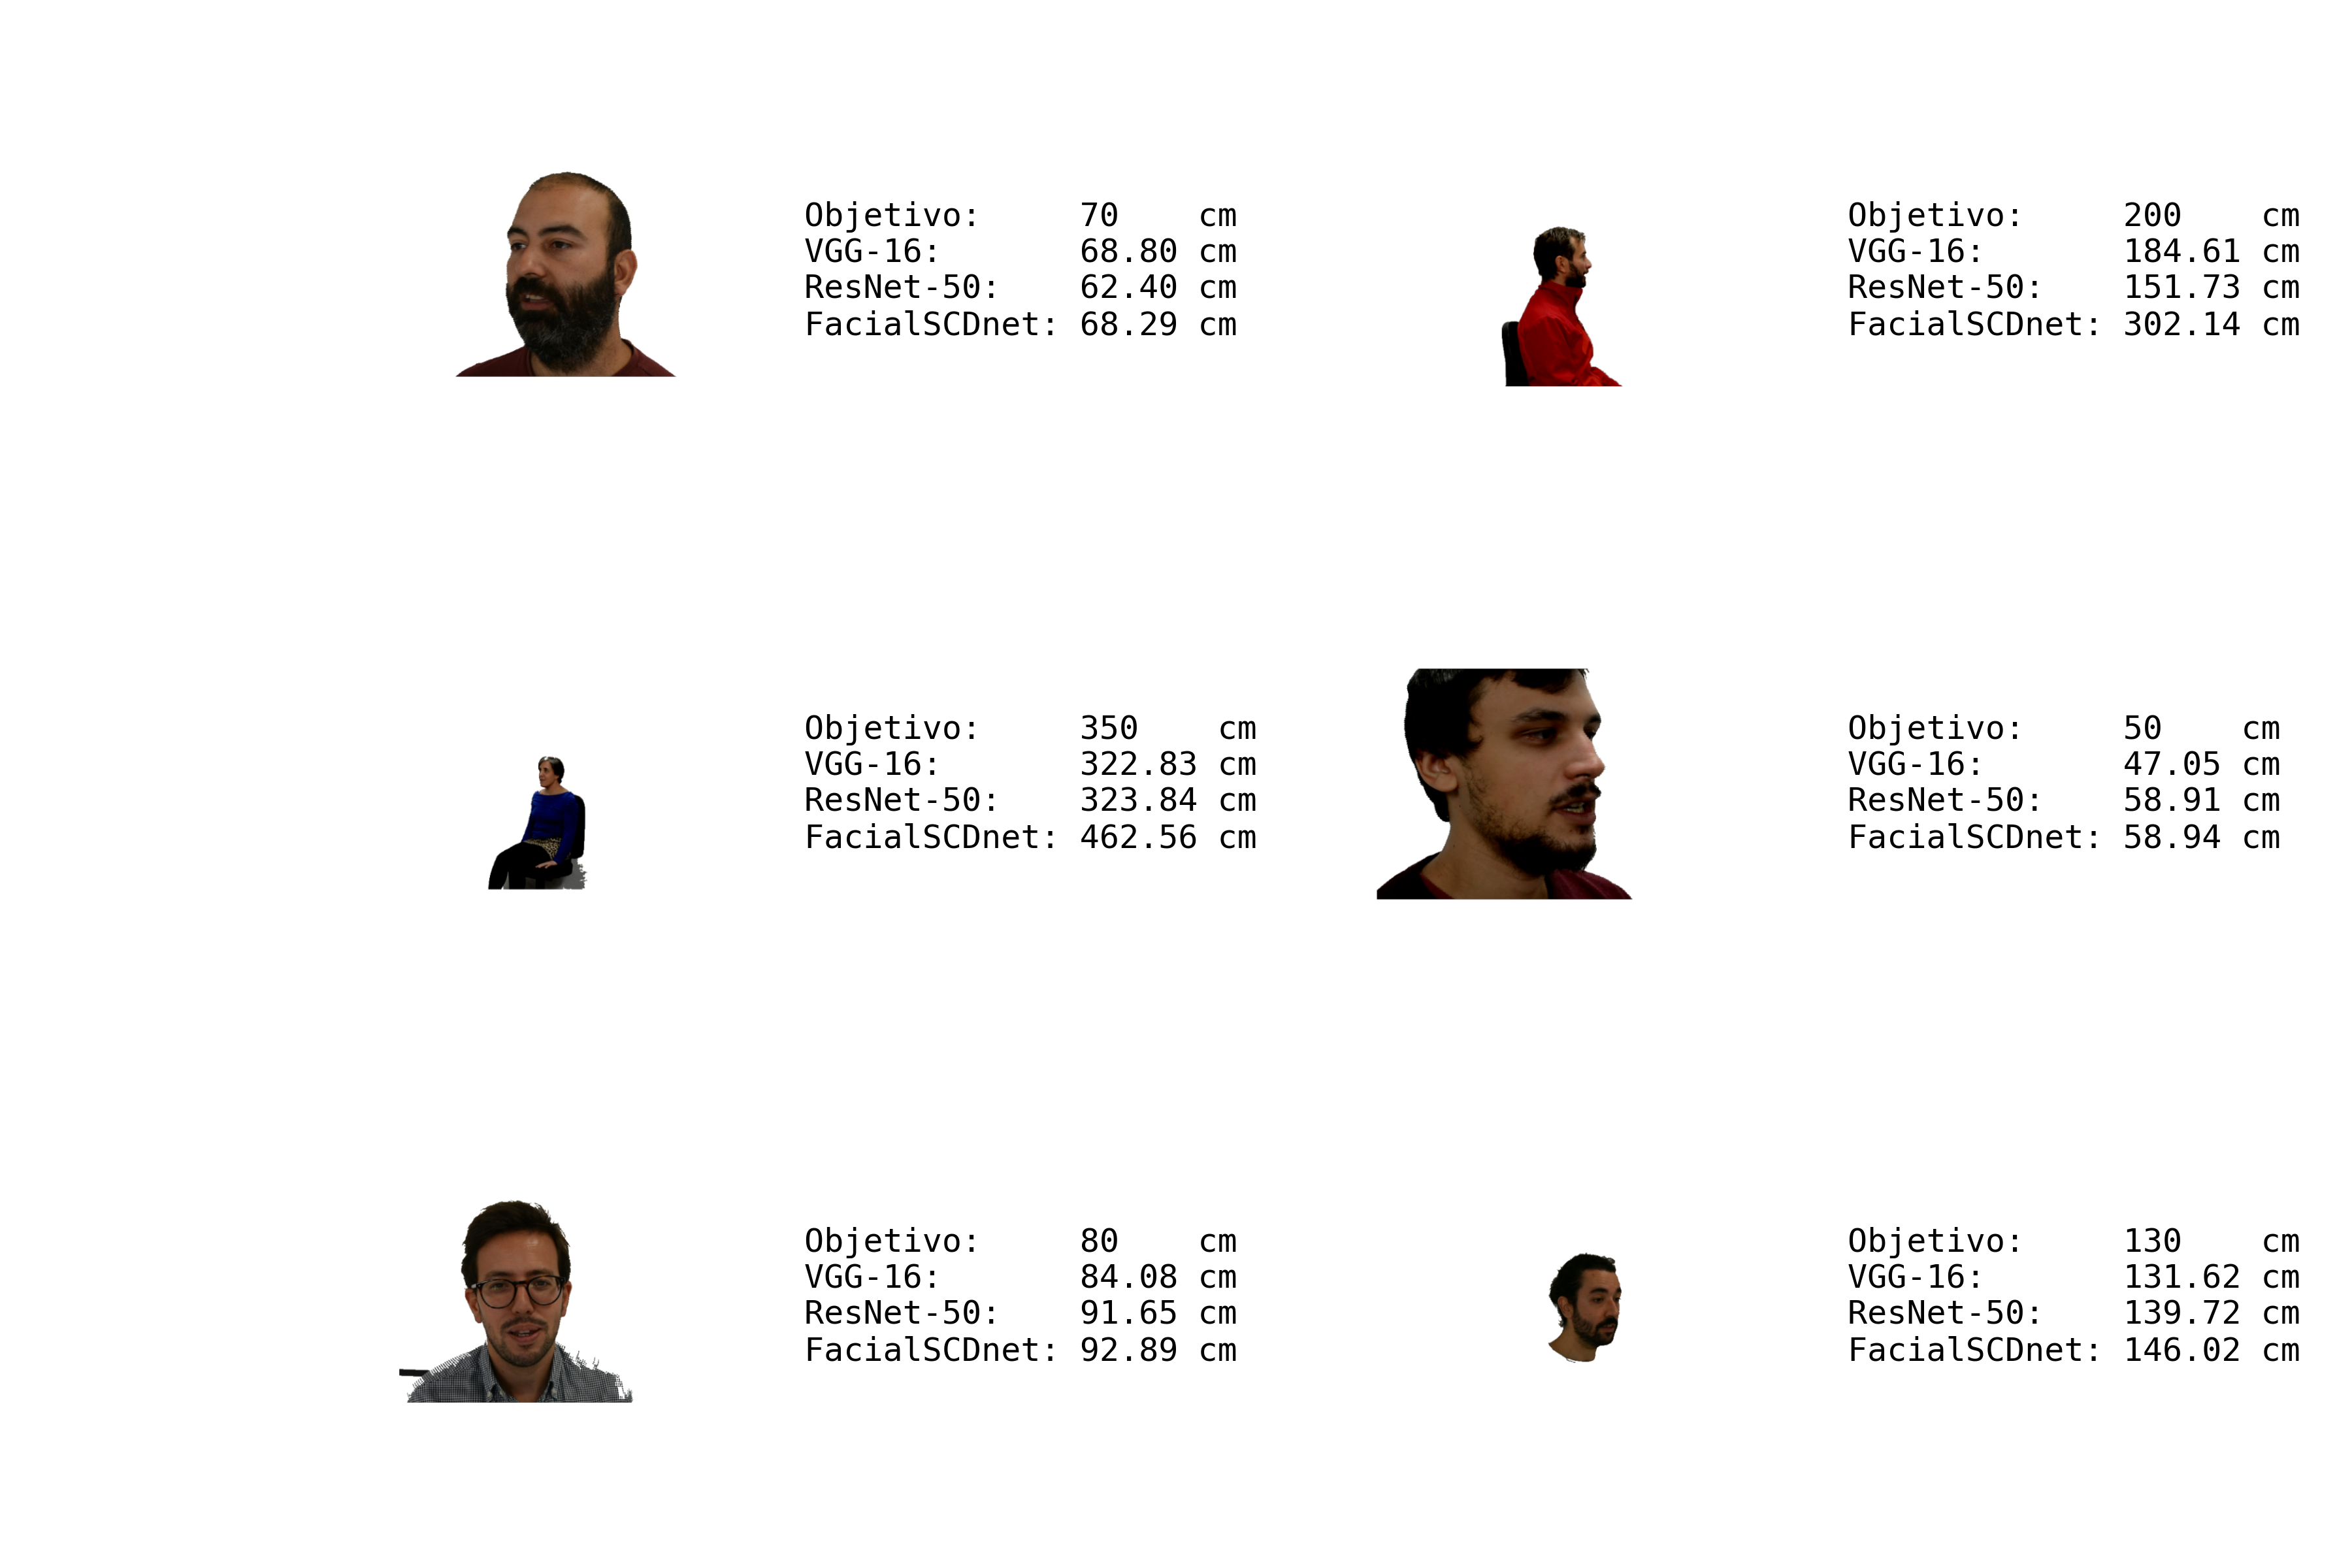
\includegraphics[width=\textwidth]{imagenes/cap5/predicts_real.png}
	\caption[Ejemplos de predicciones en imágenes reales.]{Ejemplos de predicciones en imágenes reales para los distintos modelos VGG-16 y ResNet-50 de FacialSCDnet+ y VGG-16 de FacialSCDnet.}
	\label{fig37}
\end{figure}

La Figura \ref{fig34} representa una comparativa del rendimiento de los métodos a la hora de prededir la SCD, de forma que podemos observar la dispersión concreta de las estimaciones con respecto a la SCD real. La primera fila muestra los resultados en test de los tres métodos comparados para el conjunto de imágenes sintético, mientras que la segunda fila muestra los resultados sobre el conjunto de imágenes reales. La principal diferencia entre ambos conjuntos de datos es evidente, el número de imágenes sintéticas que podemos generar permite cubrir un amplio rango de distancias en comparacion con las imágenes reales. Esto nos permite contextualizar el rendimiento de los modelos. 

\begin{figure}[h]
	\centering
	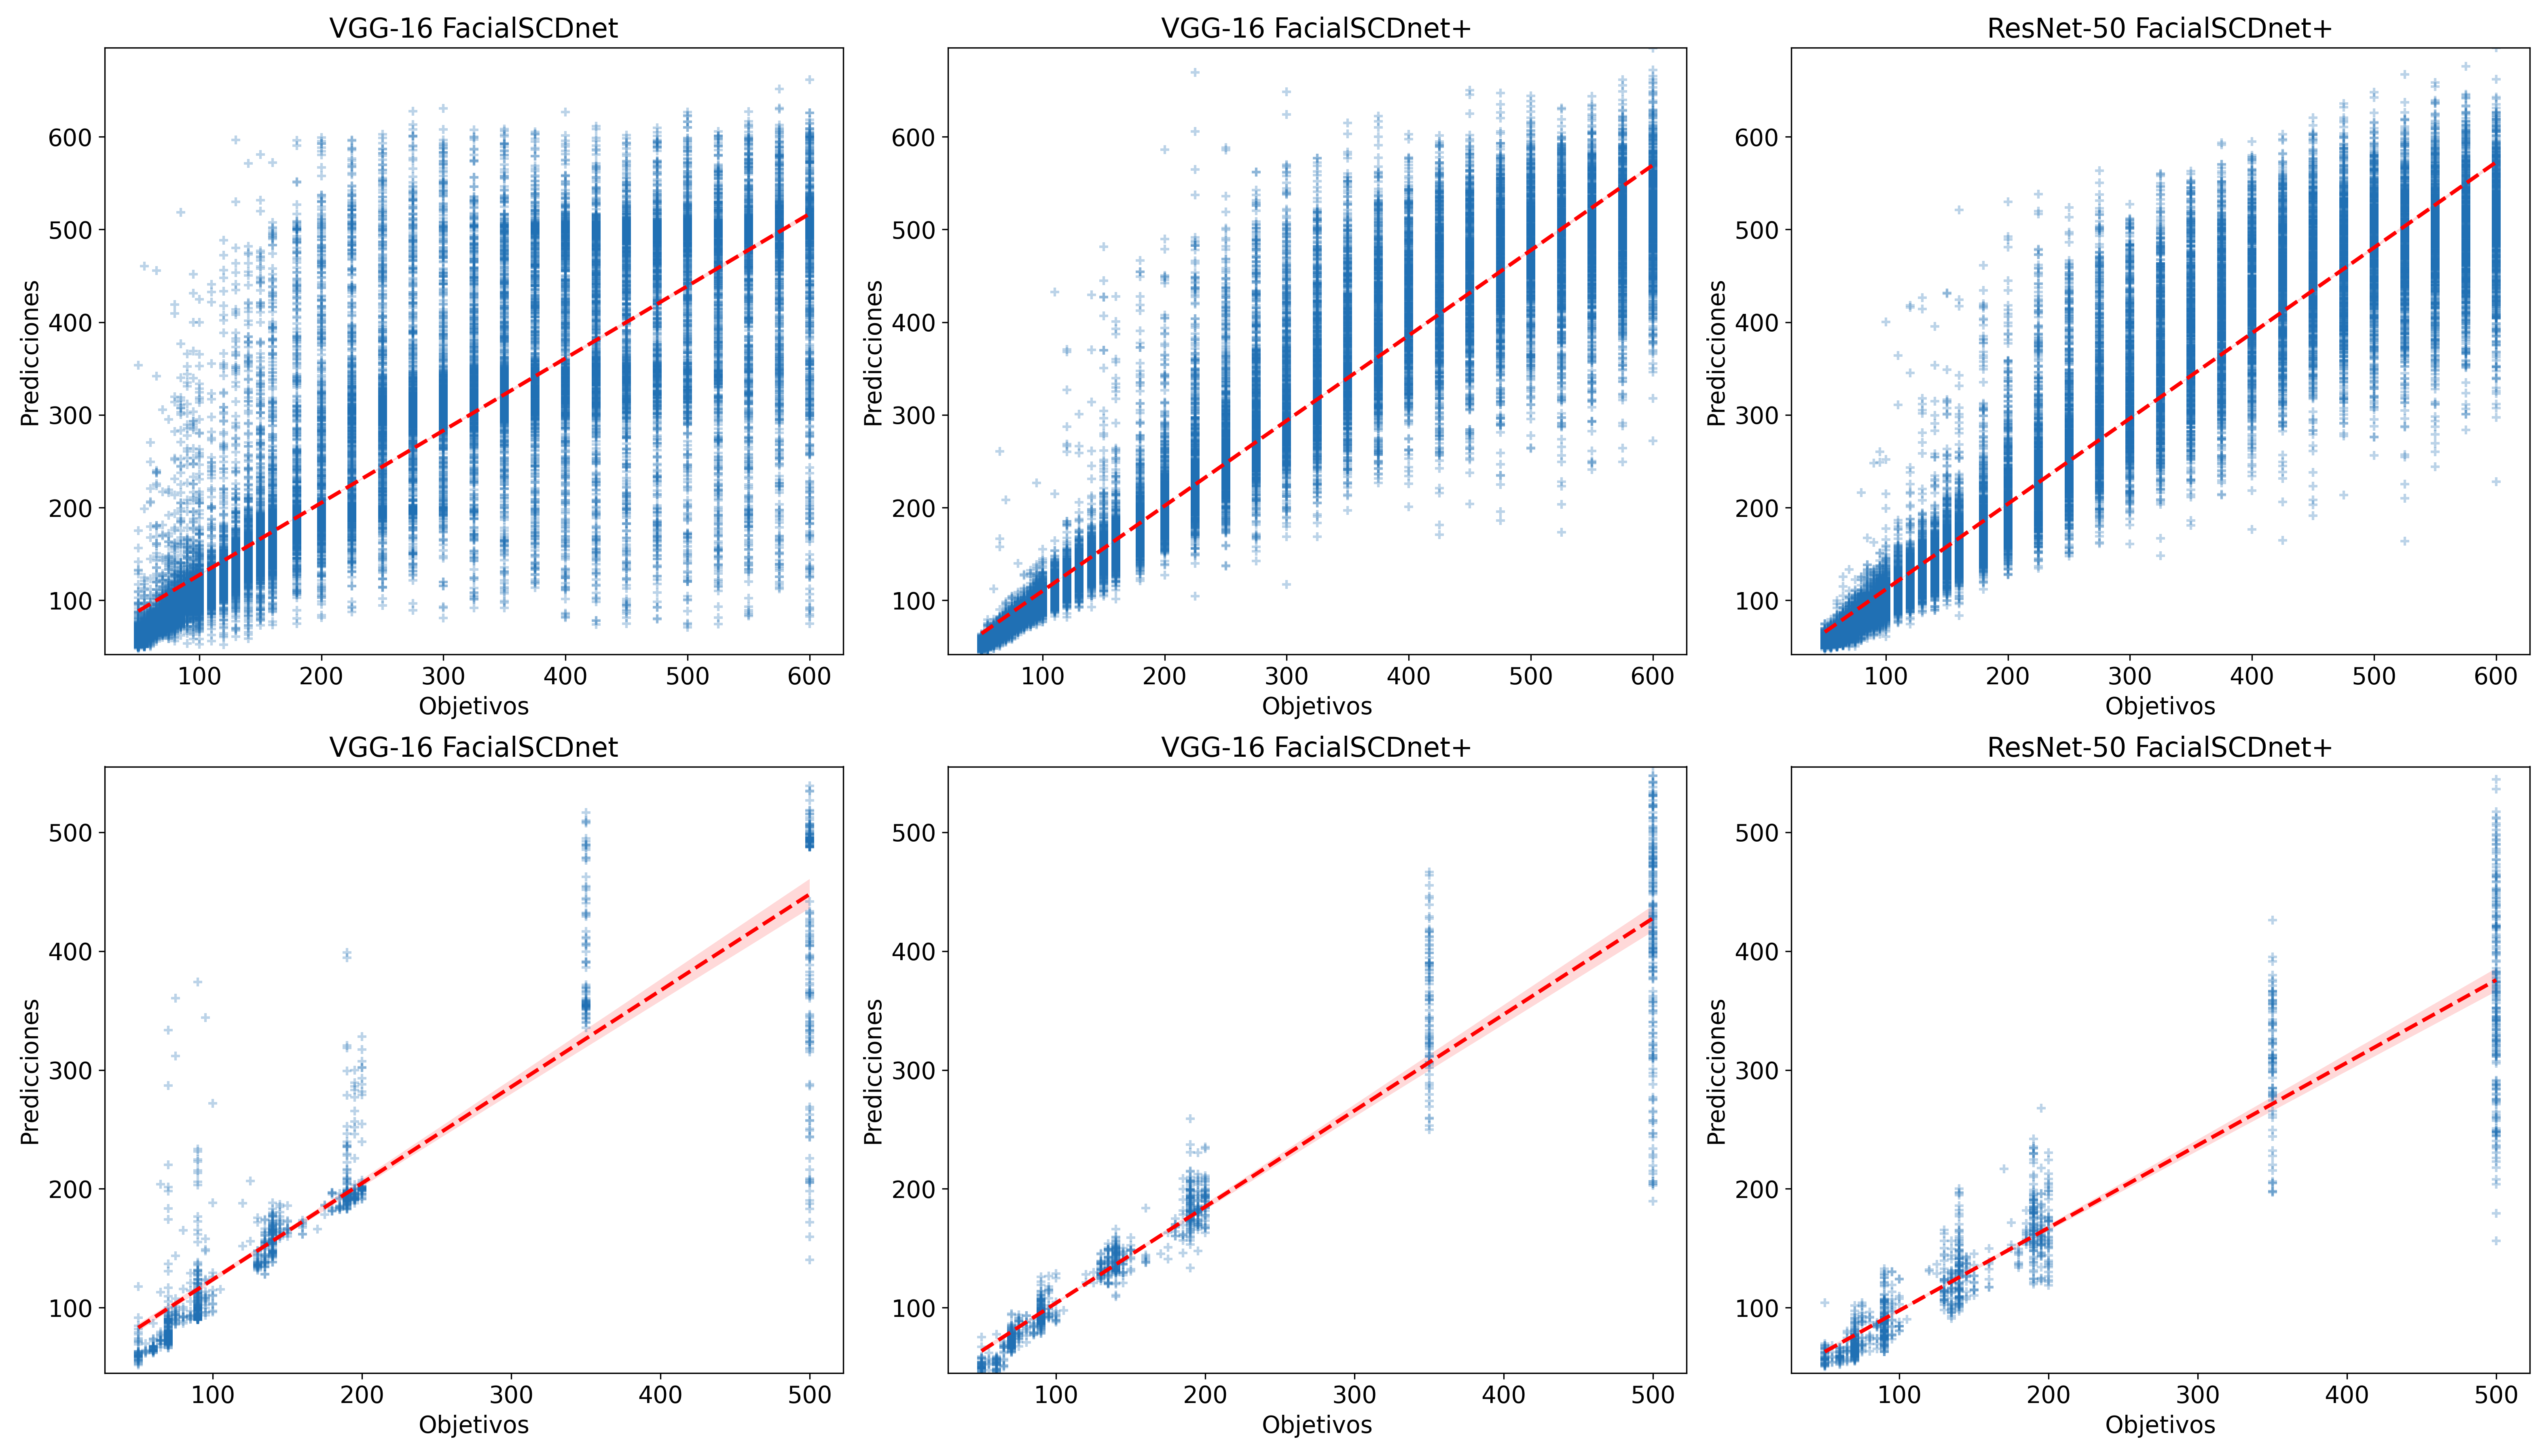
\includegraphics[width=\textwidth]{imagenes/cap5/comp_etiquetas.png}
	\caption[Comparación etiquetas de test.]{Gráfica comparativa de predicciones vs objetivos para los tres modelos utilizados. La primera fila presenta los resultados en el conjunto de test sintético, mientras que la segunda fila muestra los resultados en el conjunto de test real.}
	\label{fig34}
\end{figure}

En línea con los resultados cuantitativos mostrados en las Tablas \ref{test-mio} y \ref{test-real}, ambas arquitecturas de FacialSCDnet+ tienen un comportamiento similar, realizando estimaciones mucho más precisas a distancias cortas (en torno a 1.5 metros) y mostrando más variabilidad a distancias mayores. Es precisamente en esos casos donde el impacto de la distorsión de perspectiva es menos relevante, con lo que los resultados se explican al emplear la metrica de distorsión para guiar el entrenamiento del modelo. Para el conjunto de datos real se puede extraer una conclusión similar, destacando cómo el modelo basado en VGG-16 de FacialSCDnet+ parece minimizar la dispersión en la estimación de SCD, reduciendo los outliers y mostrando un comportamiento más consistente. En el caso del modelo de referencia, FacialSCDnet, la gráfica deja patente cómo el método, al no ser ayudado por la aplicación de las máscaras de transparencia, tiene un rendimiento real considerablemente peor al reportado en \cite{14} y del obtenido por FacialSCDnet+.

Además, los coeficientes de determinación R$^2$ (Tablas \ref{test-mio} y \ref{test-real}) proporcionan una medida cuantitativa adicional del rendimiento de los modelos, indicando qué tan bien se ajustan las líneas de regresión de la Figura \ref{fig34} a los datos. En concreto, el modelo VGG-16 de FacialSCDnet+ alcanza un valor de 0.895 para el conjunto de datos sintéticos, mientras que para el conjunto de datos reales se reduce a 0.829. Esto indica que dicho modelo tiene una buena capacidad (mayor del 80\%) para explicar la variabilidad en los datos de ambos conjuntos, mientras que el resto de modelos tienen un R$^2$ más reducido, sobre todo en el conjunto de datos real.